A proteção da \acrshort{api} de dados é bastante importante já que impede que pessoal não autorizado por esta
não efetue alterações nos dados fornecidos por esta \acrshort{api} mantendo esta informação correta e consistente.
Assim apenas pessoal autorizado poderá ler, adicionar, editar ou eliminar dados da \acrshort{api} de dados entre os
quais dados de utilizadores, de entidades, de tipologias, etc.

Além disso a necessidade de múltiplos níveis de acesso deve-se ao facto de que os utilizadores da \acrshort{api}
não devem poder efetuar as mesmas operações na \acrshort{api} de dados. Ou seja, os utilizadores devem ter diferentes permissões
onde alguns só poderão ler, outros ler e adicionar, outros ler e adicionar alguns dados, etc.

Na secção seguinte é aprofundado o \acrshort{jwt}, uma tecnologia que permite auxiliar no processo de proteção
da \acrshort{api} de dados ao tornar possível que os pedidos autorizados (com um \acrshort{jwt} válido) pela 
\acrshort{api} de dados não sejam bloqueados e que aqueles sem autorização nem permissão dada pela \acrshort{api}
de dados sejam bloqueados.

\section{Estado da Arte}

\subsection{\glsentryfull{jwt}}
O \acrshort{jwt} é um 
\textit{open standard}\footnote{Mais informação em \url{https://tools.ietf.org/html/rfc7519}} 
que define uma forma compacta e independente de transmitir com segurança informação entre partes com um objeto 
\acrshort{json}.~\cite{jwtio} 

O \acrshort{jwt} pode ser assinado digitalmente (\acrshort{jws}), encriptado (\acrshort{jwe}), assinado e depois 
encriptado (\acrshort{jws} encriptado, ou seja, um \acrshort{jwe}, ordem 
recomendada\footnote{Mais informação em \url{https://tools.ietf.org/html/rfc7519\#section-11.2}}) ou encriptado e 
depois assinado (\acrshort{jwe} assinado, ou seja, um \acrshort{jws}).

Caso seja assinado digitalmente é possível verificar a integridade da informação mas não é garantida a sua 
privacidade contudo podemos confiar na informação do \acrshort{jwt}. A assinatura pode ser efetuada através de 
um segredo usando por exemplo o algoritmo \acrshort{hmac} ou através de pares de chaves pública/privada usando 
por exemplo o algoritmo \acrshort{rsa}. No caso de se usar pares de chaves pública/privada a assinatura também 
garante que a parte envolvida que tem a chave privada é aquela que assinou o \acrshort{jwt}.

Por outro lado, os \acrshort{jwt}s podem ser encriptados garantindo a privacidade destes, escondendo a informação 
das partes não envolvidas. Nesta secção apenas se falará sobre \acrshort{jwt}s e \acrshort{jws}s (\acrshort{jwt} 
assinado). Se pretender saber mais sobre \acrshort{jwe}s pode ler o capítulo 5 do livro \textit{The JWT Handbook} 
por \textit{Sebastián E. Peyrott}.

Sendo assim, em que casos é útil o uso de \acrshort{jwt}s? 

Dois dos casos são os seguintes:
\begin{itemize}
    \item Autorização: Este será o caso para o qual o \acrshort{jwt} será usado na \acrshort{clav}. 
    Quando o utilizador realiza o \textit{login} gera-se um \acrshort{jwt} por forma a que os restantes pedidos 
    desse utilizador sejam realizados com esse \acrshort{jwt} (\acrlong{sso}). 
    O uso de \acrshort{jwt}s para estes casos permitem um \textit{overhead} pequeno e a flexibilidade de serem 
    usados em diferentes domínios;
    \item Troca de informação: No caso de troca de informação entre duas partes os \acrshort{jwt}s assinados são 
    de bastante utilidade visto que permitem verificar se o conteúdo não foi violado e, no caso de se usar pares 
    de chaves pública/privada para assinar, permitem ter a certeza que o remetente é quem diz ser.
\end{itemize}

\subsubsection{Estrutura do \glsentryshort{jwt}}

Os \acrshort{jwt}s são construídos a partir de três elementos, o \textit{header} (objeto \acrshort{json} também 
conhecido por \acrshort{jose} \textit{header}), o \textit{payload} (objeto \acrshort{json}) e os dados de 
assinatura/encriptação (depende do algoritmo usado). Estes elementos são depois codificados em representações 
compactas (\texttt{Base64 URL-safe}\footnote{Variante da codificação \texttt{Base64} onde a codificação gerada 
é segura para ser usada em \textit{URL}s. Basicamente para a codificação \texttt{Base64} gerada substitui os 
caracteres '+' e '/' pelos caracteres '-' e '\_' respetivamente. Além disso, remove o caractere de 
\textit{padding} e proíbe separadores de linha}). As codificações \texttt{Base64 URL-safe} de cada elemento 
são depois concatenadas numa \textit{string} onde é usado o caractere '.' para separar as partes, dando origem 
a uma representação final compacta do \acrshort{jwt} (\textit{JWS/JWE Compact Serialization}). 

Na secção~\ref{sec:criacaojwt} estão presentes dois diagramas referentes à construção de dois \acrshort{jwt}s 
sendo um deles assinado.

\begin{figure}[H]
    \centering
    \textbf{\textcolor{red}{eyJhbGciOiJIUzI1NiIsInR5cCI6IkpXVCJ9}.
        \textcolor{purple}{eyJuYW1lIjoiSm9zw6kgTWFydGlucyIsIm51bSI6ImE3ODgyMSJ9}.
        \textcolor{cyan}{tRPSYVsFI-nziRPuAjdGZLN2tUez5MtLML\_aAnPplgM}
    }
    \caption{Exemplo de representação compacta de \acrshort{jwt} (quebra de linhas por forma a melhorar leitura)}\label{fig:exemjwt}
\end{figure}

De seguida vamos aprofundar cada elemento referido:
\begin{itemize}
    \item[\textbf{\textit{Header}:}]

    O cabeçalho (a vermelho na figura~\ref{fig:exemjwt}) é constituído pelos seguintes atributos:
    \begin{itemize}
        \item O atributo obrigatório \texttt{alg} (algoritmo), único campo obrigatório para o caso de um 
        \acrshort{jwt} não encriptado, 
         onde é indicado que algoritmo é usado para assinar e/ou desencriptar. 
        O seu valor pode ser, por exemplo, HS256 (\acrshort{hmac} com o auxílio do 
        SHA-256\footnote{Função pertencente ao conjunto de funções \textit{hash} criptográficas 
        \acrfull{sha2} desenhadas pela \acrshort{nsa}}) ou \acrshort{rsa};
        \item O atributo opcional \texttt{typ} (tipo do \textit{token}) em que o seu valor é ``JWT''. 
        Serve apenas para distinguir os \acrshort{jwt}s de outros objetos que têm um \acrshort{jose} 
        \textit{header};
        \item O atributo opcional \texttt{cty} (tipo do conteúdo (\textit{payload})). 
        Se o \textit{payload} contiver atributos arbitrários este atributo não deve ser colocado. 
        Caso o \textit{payload} seja um \acrshort{jwt}\footnote{\acrshort{jwt} aninhado 
        (\textit{nested \acrshort{jwt}})} então este atributo deve ter o valor de ``JWT''.
    \end{itemize}

    O cabeçalho é de grande importância visto que permite saber se o \acrshort{jwt} é assinado ou encriptado e de 
    que forma o resto do \acrshort{jwt} deve ser interpretado.

    \begin{lstlisting}[language=json, caption=\textit{Header} usado para construir o \acrshort{jwt} da figura~\ref{fig:exemjwt}]
    {
        "alg": "HS256",
        "typ": "JWT"
    }
    \end{lstlisting}

    \item [\textbf{\textit{Payload}:}] O \textit{payload} (a roxo na figura~\ref{fig:exemjwt}) contém a 
    informação/dados que pretendemos transmitir com o \acrshort{jwt}. Não há atributos obrigatórios contudo 
    existem certos atributos que têm um significado definido (atributos registados).

    Existem 7 atributos registados (\textit{registered claims}):~\cite{jwthandbook}
    \begin{itemize}
        \item \texttt{iss} (\textit{issuer}): Identificador único (\textit{case-sensitive string}) que identifica 
        unicamente quem emitiu o \acrshort{jwt}. A sua interpretação é específica de cada aplicação visto que não há 
        uma autoridade central para gerir os emissores;
        \item \texttt{sub} (\textit{subject}): Identificador único (\textit{case-sensitive string}) que identifica 
        unicamente de quem é a informação que o \acrshort{jwt} transporta. Este atributo deve ser único no contexto 
        do emissor, ou se tal não for possível, globalmente único. O tratamento do atributo é específico a cada 
        aplicação;
        \item \texttt{aud} (\textit{audience}): Identificador único (\textit{case-sensitive string}) ou 
        \textit{array} destes identificadores únicos que identificam unicamente os destinatários pretendidos do 
        \acrshort{jwt}. Ou seja, quem lê o \acrshort{jwt} se não estiver no atributo \texttt{aud} não deve considerar 
        os dados contidos no \acrshort{jwt}. O tratamento deste atributo também é específico a cada aplicação; 
        \item \texttt{exp} (\textit{expiration (time)}): Um número inteiro que representa uma data e hora específicos 
        no formato \textit{seconds since epoch} definido pela 
        \acrshort{posix}\footnote{Mais informação em \url{https://pubs.opengroup.org/onlinepubs/9699919799/basedefs/V1\_chap04.html\#tag\_04\_16}}, 
        a partir da qual o \acrshort{jwt} é considerado inválido (expira);
        \item \texttt{nbf} (\textit{not before (time)}): Representa o inverso do atributo \texttt{exp} visto que é 
        um número inteiro que representa uma data e hora específicos no mesmo formato do atributo \texttt{exp}, mas 
        a partir da qual o \acrshort{jwt} é considerado válido;
        \item \texttt{iat} (\textit{issued at (time)}): Um número inteiro que representa uma data e hora especificos,
         no mesmo formato dos atributos \texttt{exp} e \texttt{nbf}, que representa o instante no qual o 
         \acrshort{jwt} foi emitido;
        \item \texttt{jti} (\textit{\acrshort{jwt} ID}): Identificador único (\textit{string}) do \acrshort{jwt} 
        que permite distinguir \acrshort{jwt}s com conteúdo semelhante. A implementação tem de garantir a unicidade 
        deste identificador.
    \end{itemize}

    Estes atributos registados têm todos 3 caracteres visto que um dos requisitos do \acrshort{jwt} é ser o mais 
    pequeno/compacto possível.

    Existem depois mais dois tipos de atributos, públicos e privados. 
    Os atributos públicos podem ser definidos à vontade pelos utilizadores de \acrshort{jwt}s mas têm de ser 
    registados em \textit{IANA JSON Web Token Claims registry} ou definidos por um espaço de nomes resistente 
    a colisões de forma a evitar a colisão de atributos. 
    Já os atributos privados são aqueles que não são nem registados nem públicos e podem ser definidos à vontade 
    pelos utilizadores de \acrshort{jwt}s. 
    Os dois atributos usados no exemplo~\ref{exem:pay} (\texttt{name} e \texttt{num}) são atributos privados.

    \begin{lstlisting}[language=json, caption=\textit{Payload} usado para construir o \acrshort{jwt} da figura~\ref{fig:exemjwt}, label=exem:pay]
    {
        "name": "José Martins",
        "num": "a78821"
    }
    \end{lstlisting}

\item [\textbf{\textit{Signature}:}] A assinatura (a azul na figura~\ref{fig:exemjwt}) é criada ao usar o 
algoritmo indicado na \textit{header} no atributo \texttt{alg} tendo como um dos argumentos os elementos 
codificados da \textit{header} e do \textit{payload} juntos por um ponto e como outro argumento um segredo. 
O resultado do algoritmo é depois codificado em \texttt{Base64 URL-safe}. 
Esta assinatura no caso dos \acrshort{jws}s é usada para verificar a integridade do \acrshort{jwt} e caso seja 
assinado com uma chave privada permite também verificar se o remetente é quem diz ser. 
No caso de o atributo \texttt{alg} for \texttt{none} a assinatura é uma \texttt{string} vazia.

    \begin{lstlisting}[language=javascript, caption=\textit{Signature} usado para construir o \acrshort{jwt} da figura~\ref{fig:exemjwt}]
    HMACSHA256(
        base64UrlEncode(header) + "." +
        base64UrlEncode(payload),
        segredo1.-uminho!clav
    )
    \end{lstlisting}
\end{itemize}

\subsubsection{Criação de \glsentryshort{jwt}/\glsentryshort{jws}}\label{sec:criacaojwt}

Na figura~\ref{fig:buildJWT} é apresentada a construção de um \acrshort{jwt} em que o atributo 
\texttt{alg} (algoritmo) tem o seu valor igual a \texttt{none}, ou seja, o \acrshort{jwt} não é 
assinado nem encriptado.

\begin{figure}[H]
    \centering
    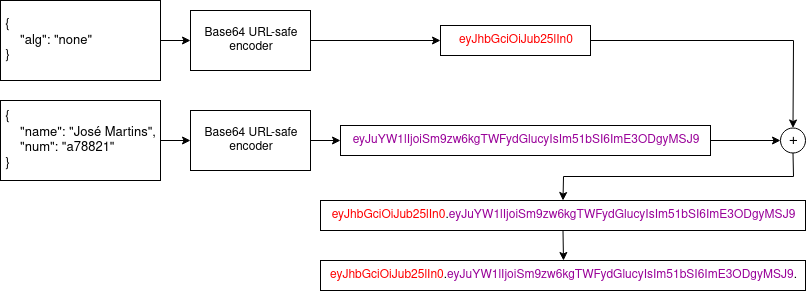
\includegraphics[width=1\textwidth]{img/buildJWT.png}
    \caption{Criação de um \acrshort{jwt}}\label{fig:buildJWT}
\end{figure}

Já na figura~\ref{fig:buildJWS} é demonstrada a construção de um \acrshort{jwt} assinado, ou seja, um \acrshort{jws}.

\begin{figure}[H]
    \centering
    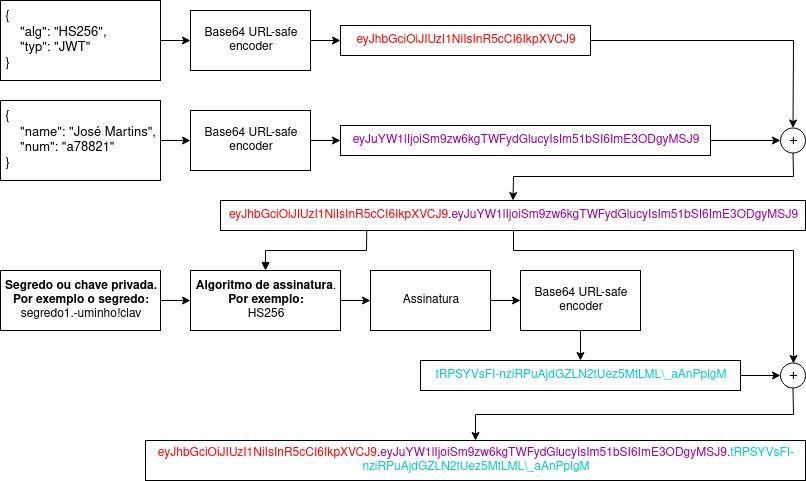
\includegraphics[width=1\textwidth]{img/buildJWS.png}
    \caption{Criação de um \acrshort{jws}}\label{fig:buildJWS}
\end{figure}

\subsubsection{Alternativas ao \glsentryshort{jwt}}

Algumas alternativas ao \acrshort{jwt} passam pelo uso de \acrfull{swt} ou \acrfull{saml}. 
Se compararmos o \acrshort{jwt} ao \acrshort{saml}, o \acrshort{json} é menos verboso que o 
\acrshort{xml} e mesmo quando codificado o seu tamanho é menor. 

De um ponto de vista de segurança o \acrshort{swt} apenas pode ser assinado simetricamente por um segredo 
partilhado usando o algoritmo \acrshort{hmac}. Já o \acrshort{jwt} e o \acrshort{saml} podem usar pares de 
chaves pública/privada para assinar. Contudo assinar \acrshort{xml} com 
\textit{\acrshort{xml} Digital Signature} sem introduzir buracos de segurança é mais difícil quando comparado 
com a simplicidade de assinar \acrshort{json}.~\cite{jwtio}

Houve contudo algumas bibliotecas de \acrshort{jwt} com vulnerabilidades devido ao atributo \texttt{alg} da 
\textit{header} do \acrshort{jwt}. Havia duas situações de vulnerabilidade:
\begin{itemize}
    \item As bibliotecas ao fazer a verificação (recebe um \acrshort{jwt} e um segredo/chave pública como 
    argumentos) de um \acrshort{jwt} com \texttt{alg} igual a \texttt{none} assumiam logo que o \acrshort{jwt} 
    era válido mesmo que o segredo/chave pública fosse diferente de vazio. Ou seja, com a simples alteração do 
    atributo \texttt{alg} e com a remoção da \textit{signature} podia-se alterar o \textit{payload} do 
    \acrshort{jwt} que o servidor iria continuar a considerar que a integridade do \acrshort{jwt} não foi colocada 
    em causa mesmo que os \acrshort{jwt}s gerados pelo servidor tivessem sido assinados com um algoritmo e 
    com recurso 
    a um segredo/chave privada;

    \item As bibliotecas ao fazer a verificação seja de um algoritmo simétrico ou assimétrico apenas tinham 
    como parâmetros o \acrshort{jwt} e o segredo/chave pública. Isto gera uma segunda vulnerabilidade. Se o 
    servidor estiver à espera de um \acrshort{jwt} assinado com pares de chaves pública/privada mas receber 
    um \acrshort{jwt} assinado com \acrshort{hmac} vai assumir que a chave pública é o segredo a usar no algoritmo 
    \acrshort{hmac}. Ou seja, se se criar um \acrshort{jwt} com o atributo \texttt{alg} igual a \acrshort{hmac} 
    e a assinatura for gerada usando o algoritmo \acrshort{hmac} com o segredo a ser a chave pública, podemos 
    alterar o \textit{payload} (antes de assinar) que o servidor vai considerar que o \acrshort{jwt} não foi 
    maliciosamente alterado.
\end{itemize}

Portanto a flexibilidade de algoritmos dada pelo \acrshort{jwt} coloca em causa a segurança pelo que da parte das 
bibliotecas o atributo \texttt{alg} não deve ser considerado~\cite{jwtvuln} bem como deve ser \textit{deprecated} 
e deixar de ser incluído nos 
\acrshort{jwt}s\footnote{Ver \url{https://gist.github.com/paragonie-scott/c88290347c2589b0cd38d8bb6ac27c03}}. 

A biblioteca que será usada na \acrshort{clav}, 
\texttt{jsonwebtoken}\footnote{Ver \url{https://www.npmjs.com/package/jsonwebtoken}}, já endereçou estes 
problemas\footnote{Ver \url{https://github.com/auth0/node-jsonwebtoken/commit/1bb584bc382295eeb7ee8c4452a673a77a68b687}} 
pelo que estas vulnerabilidades não estarão presentes na \acrshort{clav}.

Ainda comparando as diferentes alternativas, os \textit{parsers} de \acrshort{json} são mais comuns em grande 
parte das linguagens de programação visto que os \acrshort{json}s mapeiam diretamente para objetos ao contrário 
do \acrshort{xml} que não tem um mapeamento natural de documento para objeto.~\cite{jwtio} 
Isto torna mais fácil trabalhar com \acrshort{jwt} do que com \acrshort{saml}.

Já quando comparamos os \acrshort{jwt}s a \textit{cookie sessions}, o \acrshort{jwt} tem a vantagem de as sessões 
puderem ser \textit{stateless} enquanto que as \textit{cookies} são \textit{statefull}. Contudo, 
ser \textit{stateless} não permite por exemplo que a qualquer altura se possa revogar um \acrshort{jwt}. 
Para endereçar esse problema é necessário, por exemplo, guardar (\textit{statefull}) os \acrshort{jwt}s numa base 
de dados associando cada \acrshort{jwt} ao identificador único de quem é a informação contida no \acrshort{jwt} 
(o uso de uma \textit{whitelist}). Assim para revogar um \acrshort{jwt} bastaria removê-lo da base de dados.

Outra alternativa ao \acrshort{jwt} seria \textit{sessionIDs}. As \textit{sessionIDs} são \textit{strings} longas, 
únicas e aleatórias. É possível revogar um \textit{sessionID}, ao contrário do \acrshort{jwt}, bastando para isso 
remover o \textit{sessionID} da base de dados.

Por fim, uma outra alternativa bastante semelhante ao \acrshort{jwt} é \textit{Branca}. 
\textit{Branca} usa o algoritmo simétrico \textit{\acrshort{ietf} XChaCha20-Poly1305 \acrshort{aead}} que permite 
criar \textit{tokens} encriptados com a garantia de integridade. Tem também uma região de \textit{payload} como 
\acrshort{jwt} com a única diferença é que este \textit{payload} não tem uma estrutura definida. Não necessita da 
\textit{header} visto que o algoritmo usado não varia. Em vez de usar codificação em \texttt{Base64 URL-safe} 
usa \texttt{Base62} que também é \textit{URL-safe}. Para além disso o \textit{token} gerado é geralmente de menor 
dimensão do que o gerado pelo \acrshort{jwt} sendo como tal mais compacto que o \acrshort{jwt}.~\cite{branca} 
Visto que o \textit{Branca} encripta e garante integridade de uma forma mais simples que o \acrshort{jwt} 
permite (para isso era necessário recorrer a um \acrshort{jwe} que tem no seu \textit{payload} um \acrshort{jws}), 
sendo como tal propenso a menos erros de programação. 
Contudo, o \textit{Branca} ainda não é muito conhecido nem um \textit{standard} da indústria, ao contrário do 
\acrshort{jwt}, mas não deixa de ser algo a ter em conta para o futuro. 

\section{Solução}

A proteção da \acrshort{api} de dados é bastante importante visto que impede o uso indevido de pessoal não 
autorizado, isto é, não registado. Para que um utilizador possa aceder à \acrshort{api} de dados necessita de 
criar uma Chave \acrshort{api} ou de pedir o registo de uma conta. 

A proteção da \acrshort{api} de dados da \acrshort{clav} possui os seguintes requisitos:
\begin{itemize}
    \item Todos os utilizadores devem conseguir aceder às rotas a que as Chaves \acrshort{api} dão acesso;
    \item Deve ser possível definir para cada rota quem pode aceder, Chaves \acrshort{api} e/ou utilizadores;
    \item Se numa rota apenas podem aceder utilizadores deve ser possível definir que níveis de utilizadores 
    podem aceder a essa rota;
    \item A verificação da autorização e autenticação de um pedido a uma rota é realizada a partir de um 
    \textit{token} (\acrshort{jwt});
    \item Tanto uma Chave \acrshort{api} como um \textit{token} de utilizador são um \acrshort{jwt};
    \item Uma Chave \acrshort{api} para além de ainda ser válida (não ter expirado) deve estar ainda ativa;
    \item Um utilizador desativado não pode gerar um \textit{token} de utilizador (não pode realizar 
    \textit{login});
    \item Uma Chave \acrshort{api} deve ter a validade de 30 dias;
    \item Um \textit{token} de um utilizador deve ter a validade de 8 horas;
    \item A \acrshort{api} deve conseguir distinguir uma Chave \acrshort{api} de um \textit{token} de utilizador;
    \item Não deve ser possível um utilizador fazer-se passar por uma Chave \acrshort{api} e vice-versa.
\end{itemize}

Os pedidos a efetuar à \acrshort{api} devem possuir o \acrshort{jwt} na \textit{header} 
\acrshort{http} \textit{Authorization} ou na \textit{query string} do pedido num dos seguintes campos:
\begin{itemize}[leftmargin=3cm]
    \item[\textbf{\texttt{token}}] caso seja o \texttt{token} de um utilizador:\newline
        \verb|http://example.com/path/page?token=<token>|
    \item[\textbf{\texttt{apikey}}] caso seja uma Chave \acrshort{api}:\newline
        \verb|http://example.com/path/page?apikey=<Chave API>|
\end{itemize}

Na \textit{header} \textit{Authorization} é usado o esquema de autenticação 
\textit{Bearer}\footnote{Mais informação em \url{https://tools.ietf.org/html/rfc6750}} 
com umas pequenas alterações. 

Portanto o conteúdo da \textit{header} \textit{Authorization}:
\begin{itemize}[leftmargin=2cm]
    \item Caso seja o \texttt{token} de um utilizador é:\newline
        \verb|token <token>|
    \item Caso seja uma Chave \acrshort{api} é:\newline
        \verb|apikey <Chave API>|
\end{itemize}

ao invés do esquema de autenticação predefinido do \textit{Bearer}: \verb|Bearer <token/Chave API>|.

Caso não seja respeitado nenhum destes formatos, o pedido será recusado visto que a \acrshort{api} de dados não 
consegue verificar o \textit{token}.

Com estas duas formas de enviar o \acrshort{jwt} é possível distinguir os utilizadores das Chaves \acrshort{api} 
e cumprir assim um dos requisitos. Além disso, esta divisão entre utilizadores e chaves \acrshort{api} permite 
uma mais fácil gestão dos \textit{tokens} recebidos pela \acrshort{api} bem como permite usar duas formas 
diferentes de os gerar/verificar com o possível benefício de melhorar a segurança da \acrshort{api} já que também 
permite usar dois pares de chaves pública/privada, uma para as Chaves \acrshort{api}'s e outra para os 
\textit{token}'s de utilizadores impedindo assim que um utilizador se faça passar por uma chave \acrshort{api} e 
vice-versa. Para cada par de chaves geram-se os \textit{token}s usando a chave privada e validam-se usando 
a chave pública.

Um dos requisitos é que os \textit{token}s gerados pela \acrshort{api} sejam \acrshort{jwt}s. 
Contudo poderiam ser de outro tipo, por exemplo, uma \textit{string} aleatória e única. Neste caso, o processo de envio 
dos \textit{tokens} para a \acrshort{api} manter-se-ia igual. Apenas seria alterada a forma de geração e 
verificação do \textit{token}, ou seja, uma alteração interna invisível para o utilizador.

De seguida é apresentado um diagrama com a estratégia de proteção que será implementada para cumprir os requisitos 
anteriormente enunciados:
\begin{figure}[H]
    \centering
    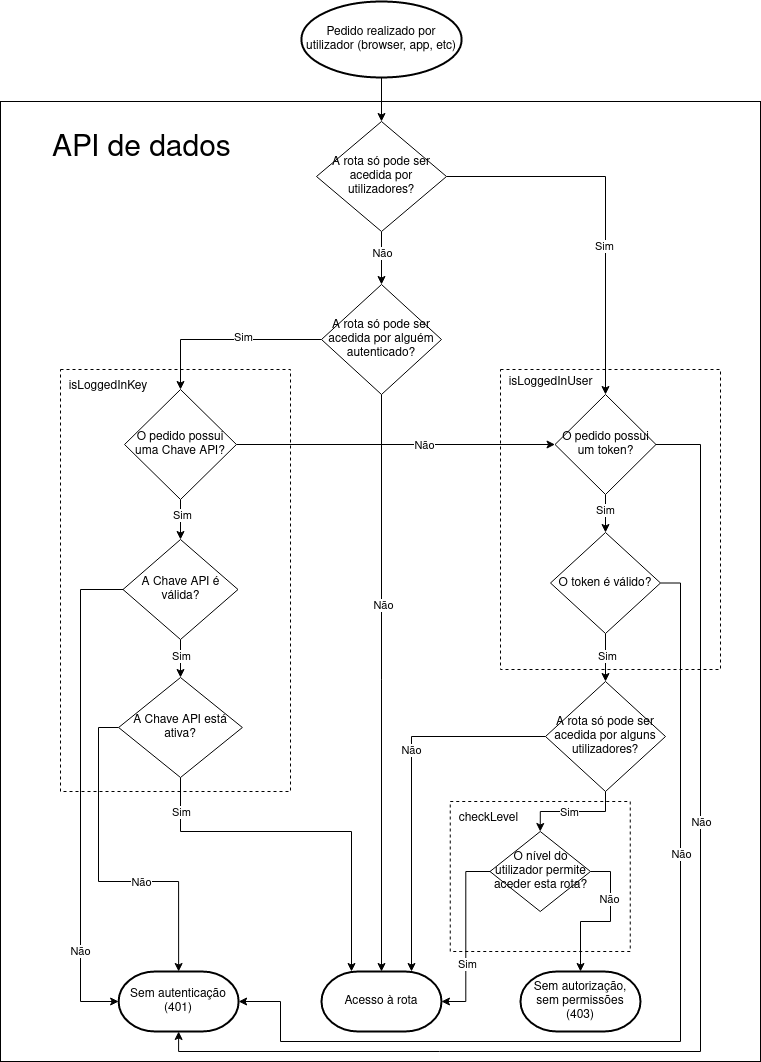
\includegraphics[width=0.7\textwidth]{img/protecaoStrag.png}
    \caption{Estratégia de proteção da \acrshort{api} de dados}\label{fig:protStrag}
\end{figure}

Como se pode observar na figura~\ref{fig:protStrag}, o \texttt{isLoggedInKey}, o \texttt{isLoggedInUser} e o \texttt{checkLevel} serão \textit{middlewares} que caso 
sejam usados numa rota definem desde logo quem pode aceder. 
Ou seja, se for usado o \texttt{isLoggedInUser} sabe-se desde logo que apenas os utilizadores podem aceder. 
Por outro lado, se for usado o \texttt{isLoggedInKey} significa que podem aceder à rota as Chaves \acrshort{api} e 
os utilizadores. Para além disso, quando o \texttt{checkLevel} é usado após o \texttt{isLoggedInUser}, sabe-se que 
apenas parte dos utilizadores pode aceder, sendo que este \textit{middleware} recebe como argumento os níveis de 
utilizadores que podem aceder à rota. A informação do nível do utilizador está presente no \acrshort{jwt} 
(\textit{token}) enviado.

Cumprem-se assim, quase todos os requisitos com a exceção dos da validade dos \textit{token}s. 
Estes são atingidos na geração dos \acrshort{jwt}'s no qual o \textit{token} de um utilizador é gerado para 
ter apenas a validade de 8 horas e uma Chave \acrshort{api} é gerada para ter a validade de 30 dias.

Após descrito como devem ser feitos os pedidos à \acrshort{api} e a estratégia de proteção a desenvolver, irão ser 
apresentados possíveis fluxos de interação entre utilizadores (\textit{browser}, \textit{app}, etc) e o 
servidor da \acrshort{api}.

O fluxo de autenticação de um utilizador na \acrshort{api} a ser implementado pode observar-se na figura~\ref{fig:userAuth}:
\begin{figure}[H]
    \centering
    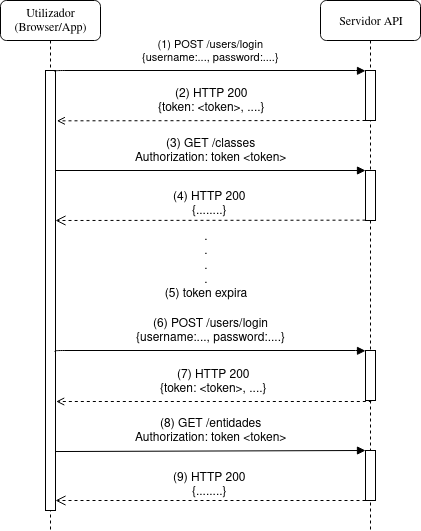
\includegraphics[width=0.5\textwidth]{img/userAuth.png}
    \caption{Fluxo de autenticação e posteriores pedidos de um utilizador}\label{fig:userAuth}
\end{figure}

\begin{enumerate}
    \item Utilizador autentica-se ao providenciar o seu \textit{email} e a sua \textit{password};
    \item Caso o utilizador se autentique com sucesso é devolvido um \textit{token} que deve ser usado nos 
    restantes pedidos até expirar;
    \item Utilizador realiza um pedido para obter as classes, colocando o \textit{token} na \textit{header} 
    \textit{Authorization};
    \item Caso o \textit{token} enviado seja válido e não tenha expirado são devolvidas as classes;
    \item \textit{Token} expirou após o tempo definido;
    \item Utilizador realiza uma nova autenticação por forma a obter um novo \textit{token};
    \item Caso o utilizador se autentique com sucesso é devolvido um \textit{token} que deve ser usado nos 
    restantes pedidos até expirar;
    \item Utilizador realiza um pedido para obter as entidades, colocando o \textit{token} na 
    \textit{header} \textit{Authorization};
    \item Caso o \textit{token} enviado seja válido e não tenha expirado são devolvidas as entidades.
\end{enumerate}

O fluxo de autenticação e renovação de uma Chave \acrshort{api} na \acrshort{api} a ser implementado pode ser 
observado na figura~\ref{fig:chaveAuth}:
\begin{figure}[H]
    \centering
    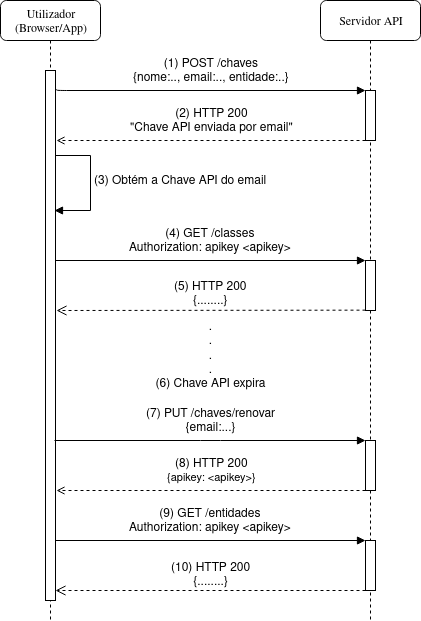
\includegraphics[width=0.5\textwidth]{img/chaveAuth.png}
    \caption{Fluxo de autenticação e posteriores pedidos de uma chave \acrshort{api}}\label{fig:chaveAuth}
\end{figure}

\begin{enumerate}
    \item Utilizador cria uma chave \acrshort{api} ao providenciar o nome, o email e a entidade a que pertence;
    \item A Chave \acrshort{api} é enviada para o email fornecido pelo utilizador com o objetivo de ser usada nos 
    próximos pedidos;
    \item O utilizador obtém a chave \acrshort{api} no email enviado;
    \item Utilizador realiza um pedido para obter as classes, colocando a chave \acrshort{api} na 
    \textit{header} \textit{Authorization};
    \item Caso a Chave \acrshort{api} enviada seja válida e não tenha expirado são devolvidas as classes;
    \item Chave \acrshort{api} expirou após o tempo definido;
    \item Utilizador renova a Chave \acrshort{api} ao providenciar o email usado para criar a Chave \acrshort{api};
    \item A nova (renovada) Chave \acrshort{api} é devolvida para ser usada nos restantes pedidos;
    \item Utilizador realiza um pedido para obter as entidades, colocando a Chave \acrshort{api} na 
    \textit{header} \textit{Authorization};
    \item Caso a Chave \acrshort{api} enviada seja válida e não tenha expirado são devolvidas as entidades.
\end{enumerate}

\section{Implementação}

Para proteger as rotas da \acrshort{api} é necessário haver métodos de verificação dos \textit{tokens} com o objetivo de decidir se o utilizador/Chave \acrshort{api} pode aceder a uma determinada rota. Isto é percetível na imagem~\ref{fig:protStrag} onde se destacam 3 \textit{middlewares}, \texttt{isLoggedInKey}, \texttt{isLoggedInUser} e \texttt{checkLevel}. De seguida será apresentado o pseudo-código destes \textit{middlewares}. 

Por forma a validar se uma Chave \acrshort{api} pode aceder a uma determinada rota é executado o \textit{middleware} \texttt{isLoggedInKey}:
\begin{lstlisting}[language=pseudocode, caption=Verificação se um pedido com uma determinada Chave \acrshort{api} pode ser efetuado]
function isLoggedInKey(req, res, next)
    key = getJWTfromHeaderOrQueryString('apikey')

    if key then
        keyBD = getKeyFromMongoDB(key)
        if keyBD then
            res = jwt.verify(key, { algorithms: ["RS256"] }, secretForAPIkey)
            if res != expired then
                if keyBD.active == True then
                    return next()
                else
                    #HTTP status 403
                    return "API Key disabled"
            else
                #HTTP status 401
                return "Unauthorized"
        else
            #HTTP status 401
            return "Unauthorized"
    else
        return isLoggedInUser(req, res, next)
\end{lstlisting}
É importante destacar a chamada da função \texttt{isLoggedInUser} que é executada no caso de não ser detetado uma Chave \acrshort{api} no pedido (na \textit{header} \textit{Authorization} ou na \textit{query string} \texttt{apikey}) e como tal, com essa chamada, tenta-se perceber se afinal foi passado um \textit{token} de um utilizador já que todos os utilizadores conseguem aceder às rotas que as Chaves \acrshort{api} conseguem como já referido.

No seguimento, para validar se um determinado \textit{token} de um utilizador pode aceder a uma determinada rota é executado o \textit{middleware} \texttt{isLoggedInUser}:
\begin{lstlisting}[language=pseudocode, caption=Verificação se um pedido com um determinado \textit{token} de um utilizador registado pode ser efetuado]
JWTstrategy = passport-jwt.Strategy

passport.use("jwt", new JWTstrategy(
    secretOrKey: secret,
    algorithms: ["RS256"],
    jwtFromRequest: getJWTfromHeaderOrQueryString('token')
, (token, done) => done(null, token)))

function isLoggedInUser(req, res, next)
    passport.authenticate("jwt", { session: false }, function (err, user, info)
        if err then
            #HTTP status 401
            return "Unauthorized"
        if !user then
            #HTTP status 401
            return "Unauthorized"
        req.logIn(user, function(err)
            if err then
                #HTTP status 401
                return "Unauthorized"

            next()
        )
    )(req, res, next)
\end{lstlisting}

Os \textit{tokens} tanto das Chaves \acrshort{api} como de \textit{tokens} de utilizadores são obtidos através da utilização de extratores presentes na estratégia \texttt{passport-jwt} do \texttt{passport}. Assim para extrair o \textit{token} da \textit{query string} basta:
\begin{lstlisting}[language=javascript, caption=Extração do \textit{token} da \textit{query string}]
var ExtractJWT = require("passport-jwt").ExtractJwt
token = ExtractJWT.fromUrlQueryParameter("<nome do campo, 'token' ou 'apikey' no caso da CLAV>")
\end{lstlisting}
Já para extrair o \textit{token} da \textit{header} \textit{Authorization} basta:
\begin{lstlisting}[language=javascript, caption=Extração do \textit{token} da \textit{header} \textit{Authorization}]
var ExtractJWT = require("passport-jwt").ExtractJwt
token = ExtractJWT.fromAuthHeaderWithScheme("<palavra antes do token, 'Bearer' no caso dum bearer token, 'token' ou 'apikey' no caso da CLAV>")
\end{lstlisting}

Para verificar se o utilizador registado tem um nível suficiente para aceder a uma rota, depois de se verificar que o utilizador está autenticado (\texttt{isLoggedInUser}), deve-se executar o \textit{middleware} \texttt{checkLevel}:
\begin{lstlisting}[language=pseudocode, caption=Verificação se um utilizador registado tem permissões suficientes para aceder a uma determinada rota]
function checkLevel(clearance)
    return function(req, res, next)
        havePermissions = False

        if clearance is Array then
            if req.user.level in clearance then
                havePermissions = True
        else
            if req.user.level >= clearance then
                havePermissions = True

        if havePermissions then
            return next()
        else
            #HTTP status 403
            return "Without enough permissions"
\end{lstlisting}
Ou seja, a variável \texttt{clearance} poderá ser uma lista de números ou apenas um número. No primeiro caso verifica-se que o nível do utilizador está presente na lista, em caso afirmativo então o utilizador tem permissões para aceder. Já no segundo caso, o utilizador só terá permissões para aceder se o seu nível foi igual ou superior ao \texttt{clearance}.

Com estes três \textit{middlewares} é possível proceder à proteção da \acrshort{api} da \acrshort{clav} garantindo que utilizadores com diferentes níveis de acesso apenas conseguem aceder ao que lhes é permitido.

\subsection{Interface da \glsentryshort{clav}}

A interface tem vários objetivos, um deles é a disponibilização de várias informações de forma pública. Com a proteção da \acrshort{api} de dados, é obrigatório em quase todas as rotas o uso de uma Chave \acrshort{api} ou de um \textit{token} de utilizador o que impossibilita a disponibilização de dados de forma pública a partir da interface. Para contornar este obstáculo, criou-se uma Chave \acrshort{api} específica para a interface para esta puder realizar pedidos à \acrshort{api}. O único problema agora é, como a interface de cada cliente irá obter a Chave \acrshort{api}?

A solução passa pela criação de uma rota específica na \acrshort{api} de dados (GET \path{/chaves/clavToken}) que caso o \texttt{Origin} do pedido seja uma das interfaces da \acrshort{clav} devolve a Chave \acrshort{api} da \acrshort{clav}. Esta rota internamente, cria a Chave \acrshort{api} caso não exista, renova-a se já tiver expirado e por fim devolve-a. Assim apenas permite-se a obtenção desta Chave \acrshort{api} pelas interfaces (através do cabeçalho \texttt{Origin}) e permite-se disponibilizar na interface de forma aberta várias informações obtidas a partir da \acrshort{api}. A Chave \acrshort{api} na interface é armazenada em \textit{localStorage}. Na \acrshort{api} de dados há uma variável, \texttt{interfaceHosts}, para definir os domínios válidos das interfaces.

Para além da proteção na \acrshort{api} de dados é necessário a proteção na interface com o objetivo de impedir o acesso indevido de utilizadores a certas páginas da interface, naquelas em que não lhe são destinadas por alguma razão bem como aquelas em que um dos pedidos à \acrshort{api} de dados irá falhar por falta de permissões. Para tal, como a interface é criada em \textit{Vue.js} podemos associar a cada rota da interface (página) um meta valor \texttt{levels} com os níveis de quem pode aceder. Estes níveis vão de 0 a 7 e o 0 indica que qualquer pessoa pode aceder (sem proteção ou Chaves \acrshort{api}) e de 1 a 7 são os níveis de utilizadores iguais aos presentes na proteção da \acrshort{api} de dados. Com este meta valor, sempre que a rota da interface muda é verificado se o utilizador pode aceder à rota, ou seja, se tem autenticação (caso necessário) e/ou autorização (caso necessário). Caso não tenha autorização o utilizador é redirecionado para a página inicial da interface e é devolvida uma mensagem de falta de permissões, mantendo o utilizador autenticado. Já no caso de falta de autenticação o utilizador é redirecionado para a página de autenticação e devolve uma mensagem de falta de autenticação tendo como possíveis razões não estar autenticado ou o \textit{token} ter expirado. Convém acrescentar que o \textit{token}, o nome e a entidade do utilizador são armazenados em \textit{localStorage}.

Ainda na interface foram feitas algumas melhorias de segurança e performance na realização dos pedidos à \acrshort{api} de dados. Por forma a evitar com antecedência pedidos que já se sabe que irão falhar por falta de autenticação o que se faz é verificar o \textit{token} antes de efetuar qualquer pedido à \acrshort{api} de dados. Isto é possível porque para gerar os \textit{tokens} são usados pares de chaves pública/privadas. Assim, para realizar esta verificação a interface apenas necessita de ter as chaves públicas. Em termos técnicos foi criado um \textit{plugin} \textit{Vue.js} que acrescenta o método \texttt{request} à \textit{framework} que deve ser usado para efetuar os pedidos à \acrshort{api} de dados, sendo que este método trata de tudo o que é necessário para realizar os pedidos, desde obter o \textit{token} do \textit{localStorage}, colocar o \textit{token} de forma apropriada no pedido a efetuar, bem como trata da verificação do \textit{token} antes de efetuar o pedido. No caso do \textit{token} de um utilizador expirar este é redirecionado para a página de autenticação enquanto que no caso da Chave \acrshort{api} da interface expirar pede de novo a Chave \acrshort{api} à \acrshort{api} pela rota anteriormente referida (GET \path{/chaves/clavToken}). Depois do pedido ser realizado, este método também faz \textit{parse} de parte dos erros, ou seja, quando a resposta do pedido tem \acrshort{http} \textit{status} 401 ou 403 este método redireciona o utilizador e devolve uma mensagem de erro de acordo com o \acrshort{http} \textit{status}. Portanto quando é 401 e o utilizador estava autenticado o utilizador é redirecionado para a página de autenticação com uma mensagem de falta de autenticação. Se for uma Chave \acrshort{api} é redirecionado para a página inicial com uma mensagem de erro para tentar de novo. Já quando é 403, este caso apenas acontece com utilizadores autenticados, o utilizador é redirecionado para a página inicial com uma mensagem de erro de falta de permissões, mantendo o utilizador autenticado. No caso de o \acrshort{http} \textit{status} não ser um destes o erro é devolvido à função que chamou este método. Assim quem desenvolve a interface não precisa de se preocupar com estas situações nem de acrescentar sempre manualmente o \textit{token} ao pedido. Necessitam apenas de enviar os dados referentes ao pedido a efetuar (verbo, caminho, \textit{body}, \textit{query string}, etc) pelo que diminui a ocorrência de erros e facilita a manutenção do código.

Por fim, uma pequena nota, um utilizador estar ou não autenticado na interface depende apenas se o \textit{token} do utilizador ainda se encontra ou não em \textit{localStorage}. Em casos de \acrshort{http} \textit{status} 401 este \textit{token} é eliminado de \textit{localStorage} necessitando o utilizador de voltar a se autenticar para voltar a obter um \textit{token} e colocá-lo em \textit{localStorage}.

\section{Resumo}

Neste capítulo é descrito como é alcançado o objetivo de proteger a \acrshort{api} de dados da \acrshort{clav} com múltiplos niveis de acesso.
Para tal, descreveu-se a tecnologia usada, \acrshort{jwt}, passando pela descrição da solução e sua implementação onde se descreveu a proteção da interface e como esta melhora o desempenho da \acrshort{api} de dados e da própria interface.
